\documentclass[10pt,twocolumn]{article}
\usepackage{amsmath}
\usepackage{amsfonts}
\usepackage{amssymb}
\usepackage{graphicx}
\usepackage{cite}


\newcommand{\argmax}{\operatornamewithlimits{argmax}}
\newcommand{\argmin}{\operatornamewithlimits{argmin}}

\title{Handwritten Digit Classification}
\author{Ian Forbes, Xinchi Chen, Niladri Mohanty}
\begin{document}
\twocolumn[
\maketitle
\section{abstract}
We attempt to classify images of handwritten digits written on various textured backgrounds. Using a training set of 50000 images we evaluate the performance of several popular machine learning algorithms. 
\\
\\
]
\section{Introduction}
Recently character recognition technology has been used in document analysis and recognition community due to the increasing demand of converting an enormous amounts of printed or handwritten information to a digital format. Application of optical character recognition (OCR) in converting historical, technical, and economic printed documents into digital form. There are some successful implementation of optical character recognition used the in digitization of handwritten documents. This field is quite challenging due to the high variability produced by noise, different handwriting styles, and image size and quality. Real world applications like bank cheque processing counts for handwriting variability\cite {diem2013icdar}. Also new handwritten digit dataset "CVL dataset" was released \cite {liu2003handwritten}. 

A fast and effective character recognition system required to solve the handwriting recognition problems such as bank cheque, automatic form processing or postal mail sorting. It is necessary to highlight that not only high speed but an accurate system is needed for classification process in real time environments. The main problem in recognizing character is variability. The same class character can be written in different sizes and orientation angles.

For improving the performance in recognition problems, image is divided into local regions \cite {lazebnik2006beyond}. This method is known as image zoning and highly successful in computer vision field\cite {ciresan2012multi}.

Recently Convolutional Neural Networks have given the best accuracy (99.73\%) on the MNIST dataset. Ciseran et al. expanded the training and testing database, including elastic distortions. Studies proved that negligence of distortion results into low accuracy rates \cite {gil2014handwritten}. Also, it is proved that classifiers which use only digit characteristics not the full image perform poorly.

\section{Preprocessing}
We tried many different preprocessing methods in attempt to reduce image noise, sharpen the appearance of the target digit, and most importantly improve our algorithms' accuracy. The first and most basic of theses methods was to normalize all of the images to a $[0,1]$ scale. The reason for this decision was that while browsing through the images we noticed that many were mostly gray with very little black or white. We believed that by normalizing the images there would be more contrast between the digit and the background which would make it easier to identify the digit. While normalization proved promising in validation, increasing our validation accuracy by roughly 1\%, our actual Kaggle submissions scored lower than the un-normalized submission.

Another basic method to reduce noise from any signal is to average it across many samples.  We tried to average all images for the same class to get rid of noise. However as the noise (texture) is random, we found it was not a great way to reduce the noise.

Another method we tried was image sharpening. Image sharpening works by subtracting a blurred copy of the image from a weighted version of the original image. The final sharpened image in our case was create by the formula: \[\text{sharpened} = 1.5 \cdot \text{original} - 0.5 \cdot \text{blurred}\]
Unfortunately this method showed no improvement over the non-sharpened images.

We also tried edge detection via the Laplacian operator $\Delta f$ (shown below) which is the sum of the second derivatives. In order to calculate the the Laplacian the original image is convolved with the image filter (kernel)  below.
\[\Delta f = \frac{\partial^2 f}{\partial x^2} + \frac{\partial^2 f}{\partial y^2}
\qquad
\begin{bmatrix}
0 & 1 & 0 \\
1 & -4 & 1 \\
0 & 1 & 0
\end{bmatrix}
\]
This operation finds areas of the image where image intensity changes rapidly. The intuition being that fast changes in image intensity indicate edges. The problem with this approach however is that the image data becomes very sparse as the majority of the images tends to zero since there is little variation in much of the image. In order to remedy this we attempted to dilate the edges by one pixel. While this worked for images with smooth backgrounds it often caused those with noisy or rough backgrounds to become completely white since the background texture was also dilated. This method therefore reduced the performance of our algorithms.

In additional to applying various image filters we also attempted to increase the amount amount of data available us by adding rotated copies of the original data to our dataset. Since the digits from the original test were rotated at random we believed this would increase the amount to useable data and therefore are test results.

The Median filter can also be used to filter the noise. Again, it did not yield any considerable differences than raw images. Therefore, we did not focused on this technique of preprocessing.
\section{Feature Selection}
For the majority of our algorithms we used the raw pixel values. However we also tried some  more complex methods to extract features from the image data.

\cite{Maji09fastand} Blockwise histograms of local orientations is used to recognize objects. This is called Pyramid Histogram of Oriented Gradients (PHOG). Each pixel in the image is assigned an orientation and magnitude based on the local gradient. Following this histograms are constructed by aggregating the pixel responses within cells of various sizes. The grayscale input image is convolved with filters which respond to horizontal and vertical gradients from which the magnitude and orientation is computed. The orientation could be signed (0−360) or unsigned (0−180). The signed gradient distinguishes between black to white and white to black transitions which might be useful for digits. PHOG features are tested with Support Vector Machine (SVM) linear and Gaussian kernel. 
\section{Algorithms}
\subsection{Naive Bayes}
Naive Bayes is a basic machine learning algorithm based on Bayes rule that can be used for multiclass classification. It uses Bayes rule along with the assumption that all features are conditionally independent given the class. The decision rule for Bayes rule is given by:
\[ \argmax_c \Pr(C = c) \prod_{i=0}^{n} \Pr(F_i = f_i | C = c)\]
We used a variant of Naive Bayes called Multinomial Naive Bayes. This method creates a Multinomial probability distribution for each feature given the class. Mathematically speaking we estimate the distribution $\Pr(F_i = f_i | C = c)$ over each of the features $f \in F$ and each class $ c \in C$ using our training data. Then we use the decision rule to find the class $c$ which maximizes this probability when classifying a test example.

In order to model the probability distributions of $\Pr(F_i = f_i | C = c)$ as a multinomial distribution we needed to discretize the the continuous $[0,1]$ values present in the images to integer values. In order to do this we created

Ideally the number of bins $B$ would be extremely large so that pixels wpubld be assigned to bins with very fine precision. The goal being to exactly replicate continuous distribution perfectly. However this would require near infinite data to construct. Because of this we need to select $B$ very carefully. To small and we loose information, to large and our histogram becomes to sparse. 

In order to select $B$ we performed 10 fold cross validation. We found that values less than $B=15$ provided poor results while for $ 15 < B < 50$ the performance was roughly the same.
\begin{figure}
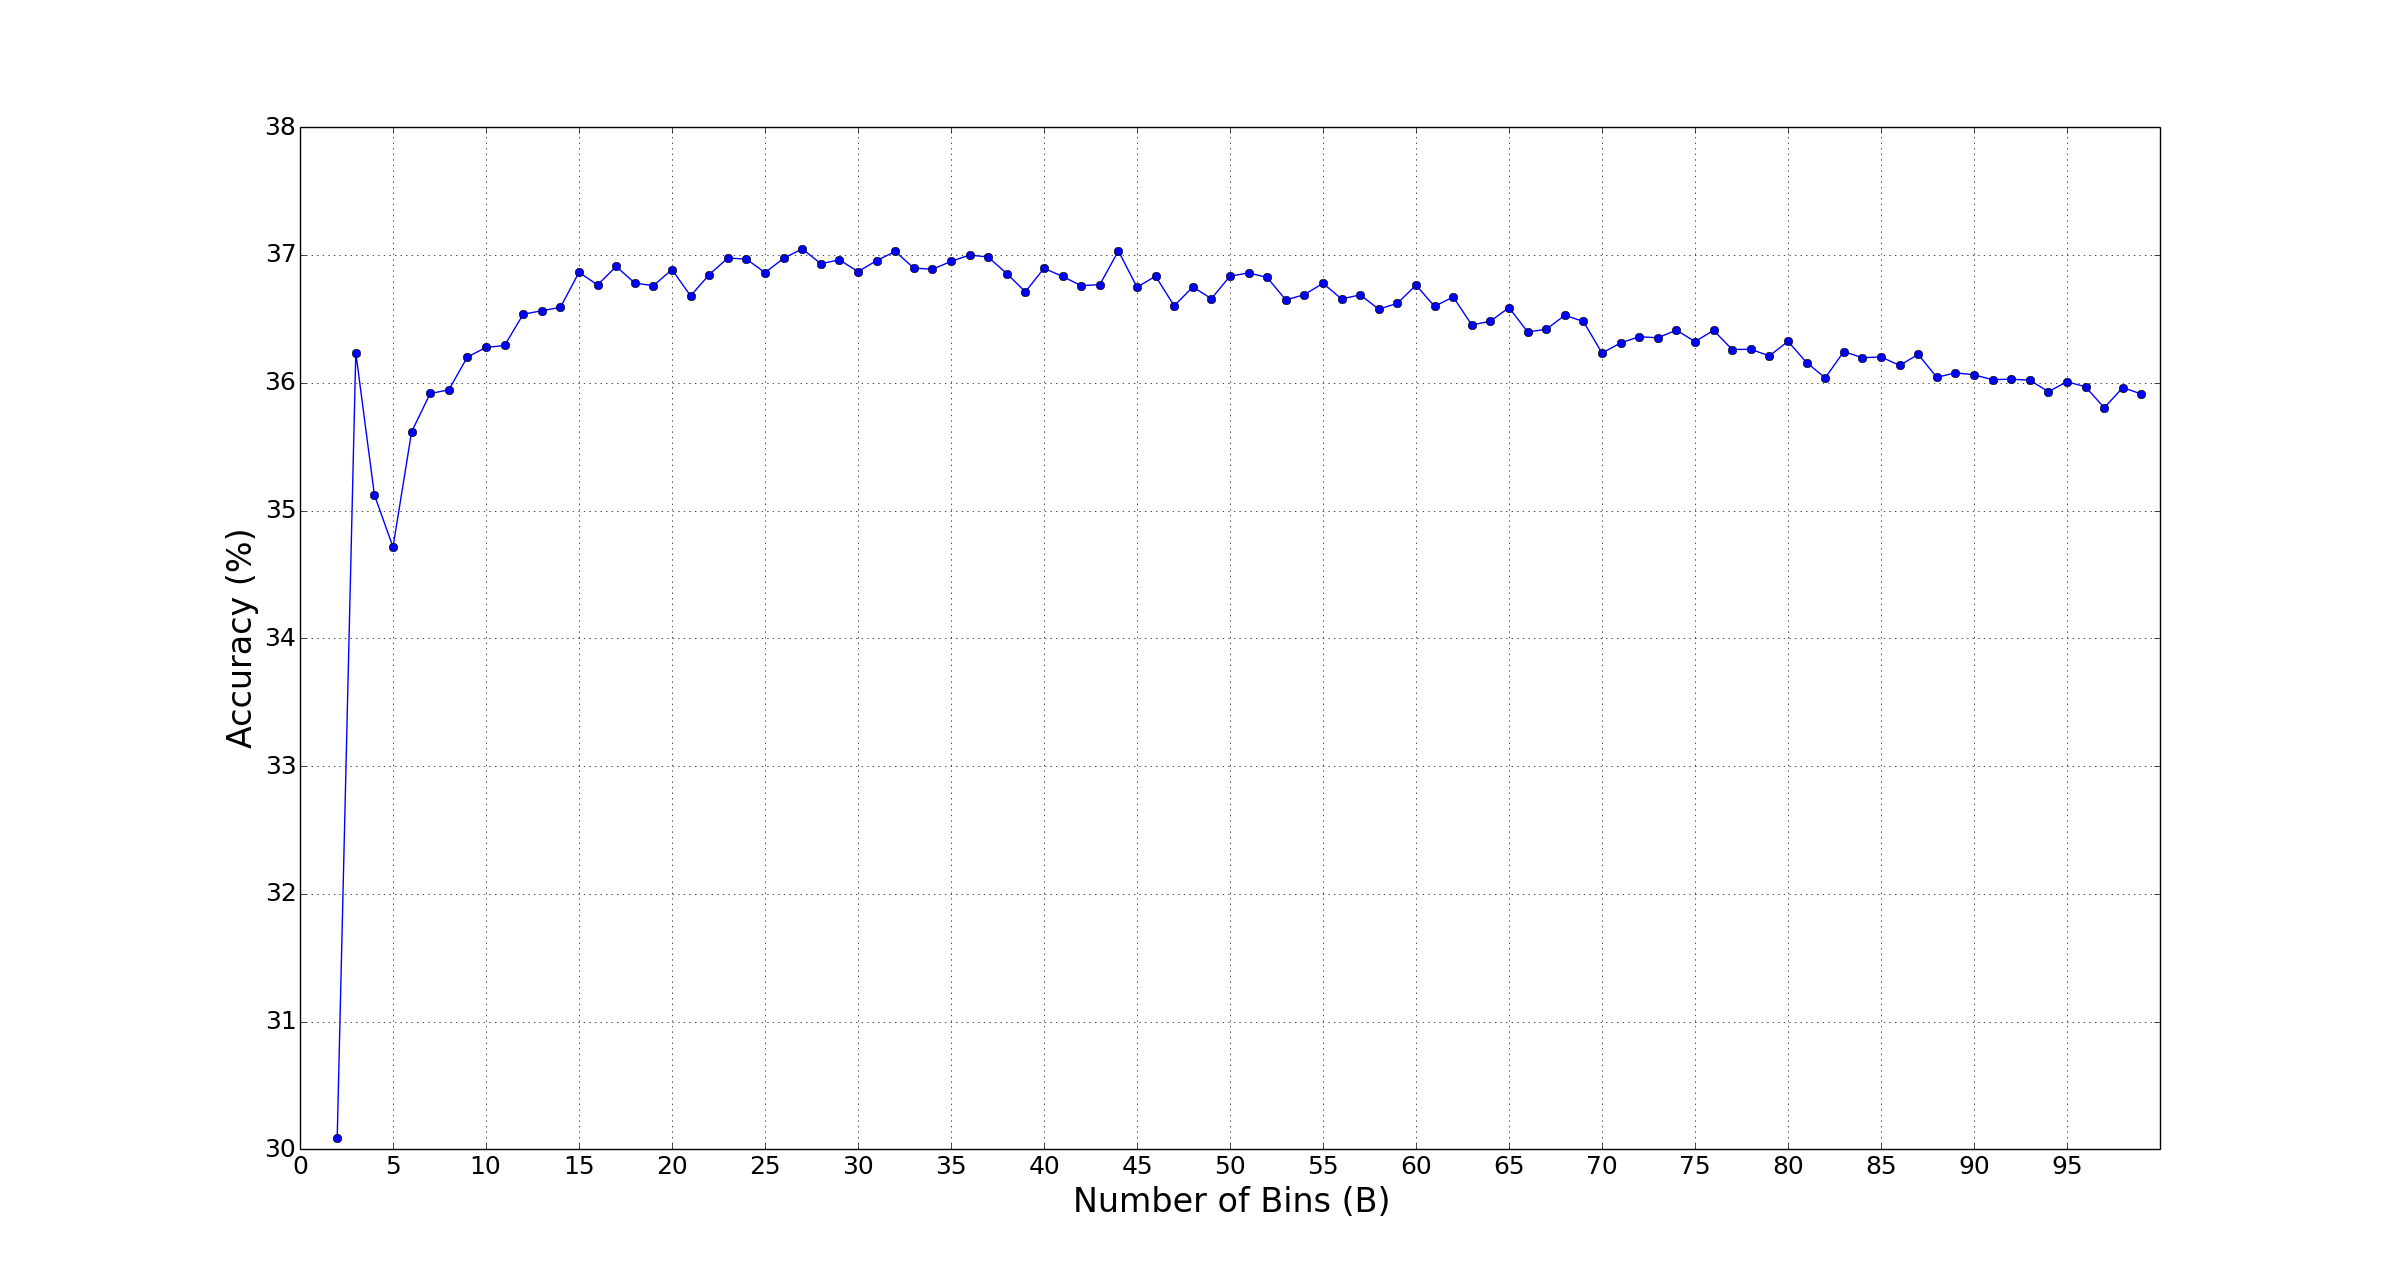
\includegraphics[trim=150 50 150 50,clip=true,width=0.5\textwidth]{./figure_1.png}
\label{bins}
\caption{Naive Bayes Accuracy as a function of the number of bins $B$. The best value of $B$ was found to be 27.}
\end{figure}
\subsection{Neural Network}
\subsection{Support Vector Machine}
Support vector machines (SVMs) have been a promising tool for data classification. Its basic idea is to map data into a high dimensional space and find a separating hyperplane with the maximal margin.

We already discussed different feature selection strategies. Combination of features and SVM is used to classify using SVM classifier \cite {chen2006combining}. In all cases, model selection was performed using a validation set. Linear SVM is used to classify test dataset. One vs all classification approach is used for multi class SVM classification. Validation accuracy is 14.63% and test dataset accuracy is 10.54%.

Linear SVM fails to classify test dataset by PHOG features. It can be inferred that there is no linear separation between different classes.
SVM can also perform efficiently for datasets which are not linearly separated. For non-linear classification, it computes a new feature for every given example depending on proximity to landmarks. It is important to note that these landmarks are chosen to be equal to $x_i, i=1,…,m$. Given $x$, the new features are computed as-
\[f_i=\text{similarity}(x_i,l_i)\]
 
To test whether SVM is a good classifier for this kind of problem or not, we tried SVM with gaussian kernel. The gaussian kernel function is given below:

\[f_i=\exp\Big(\frac{-‖x-l_i ‖}{2\sigma^2 }\Big)\]

SVM classifier with gaussian kernel is tested with σ ranging from $10^-7$ to $1$ and C = 0.1 to $10^5$ \cite {larochelle2007empirical}. Gaussian kernel SVM results for different sigma and C is shown in table 1.

\\
\\
\begin{tabular}{|c|c|c|c|}
\hline
$\sigma$ & C &	Validation & Test Accuracy \\
\hline
$10^{-7}$  & 0.1	& 31.52\%	& 26.78\% \\
$10^{-5}$	 & 10	& 32.61\%	& 29.82\% \\
$10^{-3}$	 & $10^3$ & 29.61\%	& 26.59\% \\
1        &$10^5$ & 	24.94\% & 	17.29\% \\
\hline
\end{tabular}
\\

Table 1. PHOG features gaussian SVM result
\\

The best accuracy by SVM is 32.61% on validation dataset and 29.82% on test dataset. We concluded that PHOG features are not best suited for this kind of problem where image is combined with lot of random textures. Although, Maji et. al. obtained very low percentage of error with the same features because their images were free from any noise.

We also tested SVMs both kernels for raw data. The accuracy for validation and test datasets are shown in table 2.
\\

\begin{tabular}{|c|c|c|}
\hline
Kernel & Validation accuracy & Test accuracy \\ \hline
Linear & 42.06\% & 39.48\% \\
Gaussian & 40.24\% & 39.21\% \\
\hline
\end{tabular}
\\

Table 2. Linear & Gaussian kernel SVM result
\\

\subsection{Convolutional Neural Network}
Convolution Neural Networks take inspiration from nature. In the 1960's Hubel \& Weisel conducted a wealth research on cats and monkeys in order to try to understand the biological vision systems of the brain. Their research showed that the vision system consisted of a number of `receptive fields' which were layered on top each other. They also showed that vision at least in the first steps of the vision system where highly localized. Convolutional Neural use this notion of locality when building their neurons. Where as Fully Connected NNs accept inputs from all other neurons CNNs attempt to model the biological vision system by taking locality into account in the first layers of the network. The locals layers are then feed into a FNN at the end of the network to compute the final output. This has allowed CNNs to achieve remarkably good results in the area of image recognition. 
\subsubsection{Methodology}
In order to build our CNN we used the Caffe CNN framework\cite{jia2014caffe}. Caffe allows one to create a CNN using Google Protocol Buffers, a structured data definition language similar to XML and JSON, to define the structure of the network including convolution, pooling, and fully connected layers as well as output layers such as loss, argmax, and accuracy. Using Caffe one simply has to define their NN no coding required. Caffe will then compile this the definition file and build the network from it.

We based our final network off of the LeNet architecture \cite{leCunnGradient}. This architecture was recommend by the MNIST tutorial provided on Caffe website. Since our dataset is very similar to the MNIST dataset we believed this would be a good place to start. 

In order to train and validate the performance of our network we segmented the dataset into 5 parts. We used the first 4 segments to train network and the last segment to validate against. We did not perform cross validation as the cost of train the network was quite high. 
\subsubsection{Network Architecture}
Using the MNIST architecture as a our starting point we managed achieved achieve 86.7\% accuracy on the public Kaggle test set. By adding an additional convolutional and pooling layer we managed to increase this to 91.5\%. Next we increased the initial learning rate from 0.1 to 0.5 (a learning rate of 1 lead to NaN errors) in hopes that the previous network had fallen into a local minimum. After increasing the initial learning rate to 0.5 we scored 92.1\%. 

Adding a fourth layer posed a slight problem as each convolutional + pooling layer reduces the original input of $48 \times 48$ by slightly more than half when using a $5 \times 5$ kernel. In fact the output of the 3 layer network using 5,5,5 for kernel was a single scalar value. Because of this a fourth layer could not added. In order to remedy this we had to reduce the kernel size, and therefore the rate of input size reduction, in the proceeding layers. In the end the 4 layer network used 5,5,3,3 for its kernel sizes. Unfortunately the 4 layer network proved to be significantly worse than the 3 layer network, only scoring in the 75\% range. Because of this, and the fact that the extra layer increased the training time, we choose no to train any additional 4 layer networks.
 
\subsubsection{GPU Training}
In order to train our network we used a single nVidia GTX 860m GPU with 2GB of memory we were able to train and validate our networks to convergence in roughly 20 minutes. This allowed us to easily tune parameters and add remove layers from the network inorder to see their effect on the validation score.

Graphics Processing Units (GPUs) allow for massively parallel operations to be performed on matrices and vectors. Traditionally used for graphics processing and rendering GPUs have recently found use in the fields of image processing and recognition. 

The main utility behind using GPUs is that they employ the use of thousands of lightweight threads that run in parallel. This allows for many operations on images to be processed at the same time. GPUs usually have on the order $10^4$ threads.

\section{Discussion}
\bibliographystyle{unsrt}
\bibliography{biblio.bib}
\section*{Appendix}

\end{document}
